\documentclass[12pt]{article}

\usepackage{sbc-template}
\usepackage[ruled,vlined,linesnumbered,portuguese]{algorithm2e}
\usepackage{graphicx,url}

\usepackage[brazil]{babel}
%\usepackage[latin1]{inputenc}
\usepackage[utf8]{inputenc}
% UTF-8 encoding is recommended by ShareLaTex


\sloppy

\title{Análise de Simulações \textit{in silico} do Crescimento de Tumores Malignos em Nível Celular}

\author{Arthur Passos\inst{1}, Halersson Paris Goes\inst{1}, Fernando Concatto\inst{1}}

\address{Universidade do Vale do Itajaí (UNIVALI)\\
  Caixa Postal 360 -- CEP 88302-202 -- Itajaí -- SC -- Brasil
  \email{\{arthur.titel,halersson,fernandoconcatto\}@gmail.com}
}

\begin{document}

\maketitle

\begin{abstract}
  Cancer is one of the main causes of death in many countries around the world, and the number of new cases is predicted to increase significantly in the next few years. In this context, the mathematical modelling of the disease offers a platform for the development of experiments and the discovery of new knowledge abouts its behaviour through computational means, avoiding the need to employ organic materials. Thus, this work sought to investigate mathematical models of tumour growth, analyzing them with regards to their expressiveness as well as their ability to accurately represent the real phenomenon, taking into account the development of a simulator with limited complexity.
\end{abstract}

\begin{resumo}
  O câncer é uma das principais causas de morte em diversos países, e prevê-se que o número de novos casos aumentará significativamente no futuro próximo. Neste contexto, a modelagem matemática da doença fornece uma plataforma para a realização de experimentações e a descoberta de novos conhecimentos quanto à seu comportamento através de meios computacionais, contornando a necessidade de utilização de materiais orgânicos. Assim, este trabalho buscou investigar modelos matemáticos de crescimento de tumores malignos, analisando-os tanto em relação à sua expressividade quanto à sua capacidade de representar fielmente o fenômeno real, levando em conta a construção de um simulador de complexidade limitada. % Terminar melhor? (max 10 linhas)
\end{resumo}

\section{Introdução}

O grupo de doenças conhecido como câncer é caracterizado pelo crescimento desinibido de células anormais em um organismo, possuindo a capacidade de invadir o sistema circulatório e se espalhar para órgãos distantes. Diversos fatores podem causar o surgimento do câncer, incluindo tanto hábitos e o estilo de vida individual quanto características genéticas. Mundialmente, o câncer (também chamado de tumor maligno ou neoplasia) é a segunda causa mais frequente de morte, sendo responsável pelo falecimento de aproximadamente 9 milhões de indivíduos no ano de 2015 \cite{WHO2017,ACS2017}.

Para uma melhor disseminação das características gerais do câncer, foram propostos seis aspectos biológicos que juntos formam o princípio da diversidade de doenças neoplásicas, sendo adquiridas progressivamente durante o desenvolvimento do tumor. Elas são denominadas da seguinte maneira \cite{Hanahan2011}:

\begin{itemize}
  \item Autossuficiência em Sinais Estimuladores de Crescimento (\textit{Sustaining Proliferative Signaling}): possuir controle sobre sinais proliferativos e aumentar a frequência com que estes sinais são liberados;
  \item Evasão de Supressores de Crescimento (\textit{Evading Growth Suppressors}): capacidade de ignorar sistemas que regulam e limitam o crescimento celular, mesmo quando existe alguma anormalidade na célula ou em seus arredores;
  \item Resistência a Morte Celular (\textit{Resisting Cell Death}): resistência a mecânismos naturais que resultam na morte programada das células quando as mesmas são danificadas.
  \item Potencial Ilimitado de Multiplicação (\textit{Enabling Replicative Immortality}): ignorar o estado de senescência e crise que induz a célula à um estado não reprodutivo e morte celular, respectivamente.
  \item Indução da Angiogênese (\textit{Inducing Angiogenesis}): capacidade de criar novos vasos sanguíneos a fim de aumentar o recebimento de nutrientes e oxigênio.
  \item Mecânismos de Invasão e Metástase (\textit{Activating Invasion and Metastasis}): Propriedade metástica em um sub-grupo celular.\ldots
\end{itemize}

%http://www.cell.com/cell/fulltext/S0092-8674(11)00127-9, https://drfelipeades.wordpress.com/2014/11/13/as-seis-principais-caracteristicas-do-cancer/

% Falar sobre experimentações in vivo e as dificuldades. Ver Cancer Modeling and Simulation (e-mail Santana)
Um ciclo ideal para afirmações do desenvolvimento citado nas pesquisas, faz-se necessário observações fenomenológicas, na qual toda teoria relatada é alterada para experiências de consciência. Cientistas em medicina biológica optam por abordagens inofensivas, onde são realizadas testes \textit{in vivo}, ou seja, ratos, embriões de frangos ou \textit{in vitro}. Os resultados das experiências observáveis, tanto por meios biológicos, matemáticos ou físicos, podem gerar modelos à fins de descrever padrões de comportamento \cite{Preziosi2003}.

Os atributos da pesquisa indicam referencias para soluções matemáticas de comportamentos aprofundados do problema, logo, o retrato matemático pode ser implementado para gerar modelos \textit{in silico} do evento. Para que o modelo gerado seja aceitável, a modelagem deve ter um certo grau de refino e precisão, portanto, deve haver ciclos de comparações entre as simulações do modelo matemático com os experimentos realizados em laboratório. As simulações inversas precisam concordar com as propriedades qualitativas da solução, caso contrário, o código numérico não é suficientemente preciso e que o teor as previsões precisam concordar com as experiências, caso contrário, o modelo matemático não é satisfatório \cite{Preziosi2003}. % Esta? --sim!

% Falar sobre modelagem matemática em geral e de câncer. Ver artigos de survey
%Modelos matematicos
O propósito da modelagem matematica está relacionada com a resolução do problemas. No final do modelo, busca-se um resultado que seja a solução do prblema primario, que pode acarretar também em problemas secundários do objetivo principal. Dentre vários tipos de abordagem para a modelação matematica, a modelagem via equações diferenciais tem um dos papeis princípais nos dias atuais, pois é facilmente observável as informações sobre a taxa de variação do evento, ela vem sendo utilizada desde o século XVII para modelar fenomenos reais com grau de precisão e fidelidade considerável para fundar métodos computacionais.
Apesar dos modelos matématicos apresentarem fatores favoráveis para a contribuição da resolução de um problema, existe, consequentemente, uma demanda mais detalhada do modelo, tais como maior números de parâmetros exijidos e coêrencia nos resultados obtidos, por isso há uma necessidade de controle entre a complexidade do modelo com a realidade do problema, tal como sua interpretação.

%1modelo do cancer
O processo de criação dos modelos matemáticos do câncer é extremamente complexo pois envolve o conhecimento de diferentes áreas de conhecimento, tais como biôlogicas, medicinais, matemáticos, Além de demandar um valor inicial mais proximo do resultado real, no qual vem sendo um problema nos dias atuais.
% Aprofundar para o contexto do artigo, falando sobre o objetivo e apresentar seções (separar parágrafos se ficar grande).

Este artigo é estruturado da seguinte maneira: a Seção~\ref{sec:relatedwork} apresenta alguns trabalhos relacionados ao presente, apontando algumas das abordagens discutidas na literatura sobre a modelagem matemática do crescimento de tumores malignos; na sequência, a Seção~\ref{sec:methodology} apresenta a metodologia adotada para a construção do simulador proposto neste trabalho, explorando detalhes da implementação computacional do mesmo; subsequentemente, a Seção~\ref{sec:results} descreve e analisa os resultados obtidos através da utilização do simulador, relacionando-os com dados provenientes de outras investigações; por fim, a seção~\ref{sec:conclusions} discute sobre algumas conclusões extraídas a partir dos resultados coletados e da análise comparativa, além de comentar sobre os objetivos atingidos e sobre oportunidades para aprimoramentos.

\section{Revisão bibliográfica} \label{sec:relatedwork} % Alt: Trabalhos relacionados
Durante todos estes anos de pesquisa, vários modelos matemáticos para o Câncer foram propostos,

% Falar sobre alguns artigos relacionados, não necessariamente aqueles que acabamos utilizando. Citar outras abordagens além de equações diferenciais. Falar sobre crescimento logístico/Gompertz, etc. MUITAS citações nesta seção.
Um dos modelos adotados foi o modelo de Gompertz, no qual é denominado um modelo de serie temporal e função sigmoide(função matemática com forma de S), aonde o crescimento é mais lento no início e no final da curva. Diferente da função logística, que a borda da curva é simetrica no início e no fim, o modelo de gompertz tem uma borda de curva maior no final do crescimento do que no início. Este modelo é utilizados por várias áreas que demandam um resultado parecidos com exponenciais, tal como o crescimento do ser humano.

% CITAR: https://www.ncbi.nlm.nih.gov/pmc/articles/PMC52015/pdf/pnas01064-0099.pdf (Cornil 1991)
% >= 1 página de conteúdo.
% Modelo de Panetta
%FAZER A CITAÇÃO NO X kkk --feito!

Estudos feitos por \cite{Cornil1991} avaliam os resultados da influência de fibroblastos dérmicos normais nas células de melanomas de humanos obtidos em diferentes estágios do progresso do tumor. Foi descoberto, por experimentos \textit{in vitro}, que a maioria das linhas de melanomas derivadas do início do estágio da fase de crescimento radial ou metaestático são reprimidas por fibroblastos dérmicos normais, insinuando que o cresimento homeostático negativo ainda estão operantes nas células melanomas dos estágios iniciais da doença. Entretanto, cerca de 80\% da células melanomas derivada da metástase já avançada, foram estimadas o crescimento consistente na presença de fibroblastos dérmicos. Logo, o conjuntos de resultados obtidos indicam que fibroblastos podem ter efeitos de crescimento antiéticos e inesperados em tumores.

\begin{equation} \label{eq:normalgrowth}
  \frac{\mathrm{d} s}{\mathrm{d} t} = r_{1} s \left ( 1 - \frac{s}{K_1} - \lambda_{1} c \right )
\end{equation}

\begin{equation} \label{eq:cancergrowth}
  \frac{\mathrm{d} c}{\mathrm{d} t} = r_{2} c \left ( 1 - \frac{c}{K_2} - \lambda_{2} s \right )
\end{equation}

\begin{equation} \label{eq:normalchemo}
  s(np^{+}) = F_{1}(D) s(np^{-})
\end{equation}

\begin{equation} \label{eq:cancerchemo}
  c(np^{+}) = F_{2}(D) c(np^{-})
\end{equation}

% p: período entre doses

% Falar de alguns modelos mais obscuros como sistemas multiagentes e equações diferenciais parciais.

Neste trabalho, a modelagem de \cite{Panetta1996} foi selecionada para implementação e análise, devido à sua generalidade e semelhança em relação a abordagens relacionadas. A existência de parâmetros para o controle de cada uma de suas variáveis permite que algumas de suas características, como a competição entre células normais e cancerígenas, sejam completamente desativadas, favorecendo a comparação com modelos mais simples.

\section{Metodologia} \label{sec:methodology} % Alt: Modelos e métodos

Para atingir os objetivos definidos neste trabalho, se fez necessária a construção de um simulador computacional capaz de receber como parâmetros de entrada as variáveis do modelo adotado e gerar como saída um conjunto de triplas $(s, c, t)$, com $s$ representando o número de células saudáveis, $c$ representando o número de células cancerígenas (Equações~\ref{eq:normalgrowth} e \ref{eq:cancergrowth}) e $t$ representando o tempo decorrido em dias (com $t_{0} = 0$ e $t_{n} = T$ indicando os pontos de início e término da simulação, respectivamente).
Assim, dois parâmetros adicionais de entrada $s_{0}$ e $c_{0}$ se tornam necessários para especificar as condições iniciais do sistema, caracterizando-o como um problema de valor inicial (P.V.I.). O intervalo de tempo entre dois registros é definido pela estratégia de resolução numérica do problema, descrita na Subseção~\ref{sec:numerical}.

% Neste parágrafo estamos falando das três equações de Berenbaum 1969, então não será necessário enumerá-las na seção anterior
Como foi descrito na Seção~\ref{sec:relatedwork}, o modelo adotado utiliza as Equações~\ref{eq:normalchemo} e \ref{eq:cancerchemo} para determinar a fração de células normais e cancerígenas sobreviventes após uma dose da medicação quimioterápica.
Como escolhas para as funções $F_1$ e $F_2$, \cite{Berenbaum1969} propõe duas funções exponenciais e uma hiperbólica, com base em extensivas análises a partir de dados de experimentos \textit{in vivo}. Com o intuito de minimizar o número de parâmetros do modelo, a função exponencial $F(D) = e^{- \alpha D}$ será empregada tanto para $F_1$ e $F_2$, pois a mesma demandará dois parâmetros adicionais $\alpha_1$ e $\alpha_2$, enquanto as remanescentes demandariam quatro novos parâmetros.

\subsection{Resolução das equações diferenciais} \label{sec:numerical}

O sistema de equações diferenciais proposto por \cite{Panetta1996} para a modelagem do crescimento de tumores é composto por equações diferenciais ordinárias de primeira ordem não-lineares, devido à presença do expoente 2 nas variáveis dependentes, como pode ser verificado no termo $s(s / K_1)$ na Equação~\ref{eq:normalgrowth}. Assim, se faz necessária a utilização de métodos numéricos para a aproximação de sua solução, pois a não-linearidade torna a resolução analítica inviável.

Diversas técnicas de resolução de equações diferenciais ordinárias estão disponíveis na literatura, possuindo diversos níveis de estabilidade, precisão e complexidade. Entre as estratégias mais eminentes, se encontram o Método de Euler e os Métodos de Runge--Kutta, que consistem em generalizações do primeiro e tipicamente apresentam desempenho superior; entretanto, tal superioridade é acompanhada de uma maior dificuldade de análise e implementação \cite{Butcher2016}. Como os objetivos deste trabalho incluem o desenvolvimento de um simulador do crescimento de tumores malignos visando facilidade de compreensão e codificação, o Método de Euler foi selecionado para solucionar aproximadamente o conjunto de equações diferenciais.

O Método de Euler consiste em uma estratégia simples e direta para a resolução de equações diferencias ordinárias, sendo baseado em repetidas avaliações da função característica da equação diferencial. Dado um problema de valor inicial da forma

\begin{equation}
  \frac{\mathrm{d} y}{\mathrm{d} t} = f(y), \qquad y(t_{0}) = y_{0}
\end{equation}

\noindent com $f(y)$ representando uma função qualquer da variável $y$ e $y_{0}$ indicando a condição inicial do problema, o Método de Euler pode ser formulado da seguinte maneira \cite{Butcher2016}:

\begin{equation}
  y(t_{n+1}) = y(t_{n}) + h f(y(t_{n}))
\end{equation}

\noindent sendo que o parâmetro $h$ representa o \emph{tamanho do passo}, ou seja, o intervalo entre avaliações da função ($t_{n+1} - t_{n}$). Este parâmetro é responsável pela precisão do método; quanto mais reduzido for seu valor, menor será o erro em relação à solução exata da equação diferencial, porém maior será o esforço computacional necessário para efetuar a resolução do problema. No contexto deste trabalho, $h$ representará também o intervalo entre a criação dos registros de saída pelo simulador.

\subsection{Detalhamento do simulador} \label{sec:simulator}

O simulador computacional descrito neste trabalho foi implementado utilizando a linguagem de programação JavaScript, incluindo também um módulo de interface gráfica desenvolvido com as linguagens de marcação HTML e CSS. Para realizar a atualização dinâmica da interface gráfica ao longo da simulação, a biblioteca \emph{p5.js} foi empregada, a qual é capaz de desenhar tanto formas geométricas bidimensionais simples quanto complexos modelos de três dimensões. Na ferramenta construída, células normais foram representadas por círculos de cor verde, enquanto células cancerígenas foram caracterizadas por cículos em tons de vermelho.

A linguagem de programação JavaScript não oferece nenhum suporte para a execução de código de maneira paralela (\textit{multithreaded}); portanto, os procedimentos de atualização das variáveis do modelo e o desenho das entidades gráficas devem obrigatoriamente ocorrer de modo serial, no mesmo contexto de execução. A biblioteca \emph{p5.js} invoca continuamente uma função de nome \emph{draw()}, a qual é definida pelo desenvolvedor, para atualizar o estado do programa e, por fim, a própria tela. O Algoritmo~\ref{alg:update} apresenta o procedimento de atualização implementado neste trabalho.

\begin{algorithm}[h]
  \small
  \DontPrintSemicolon
  \caption{draw() - Atualização do Estado do Simulador}
  \label{alg:update}
  \SetKwInOut{Input}{Entrada}
 \Input{$s$, $c$, $h$}

  $\Delta s \leftarrow h * crescimentoNormal(s, c)$
  \tcp*[r]{Equação~\ref{eq:normalgrowth}}
  $\Delta c \leftarrow h * crescimentoCancerigeno(c, s)$ \tcp*[r]{Equação~\ref{eq:cancergrowth}}
  \BlankLine

  \If{$t > n * p$}{
    \tcp{Calcula quantas células morreram com a dose}
    $(M_s, M_c) \leftarrow aplicarQuimioterapia(s, c)$ \tcp*[r]{Equações~\ref{eq:normalchemo} e \ref{eq:cancerchemo}}
    \BlankLine

    $\Delta s \leftarrow \Delta s - M_s$ \;
    $\Delta c \leftarrow \Delta c - M_c$ \;
    \BlankLine

    $n \leftarrow n + 1$ \;
  }
  \BlankLine

  $Z_s \leftarrow Z_s + \Delta s$ \;
  $Z_c \leftarrow Z_c + \Delta c$ \;
  \BlankLine

  \tcp{Cria células se os valores forem positivos}
  \tcp{e remove caso contrário}
  $atualizarCelulas(floor(Z_s), floor(Z_c))$\;
  \BlankLine

  $Z_s \leftarrow Z_s - floor(Z_s)$ \;
  $Z_c \leftarrow Z_c - floor(Z_c)$ \;
  \BlankLine

  $s \leftarrow s + \Delta s$ \;
  $c \leftarrow c + \Delta c$ \;
  \BlankLine

  $t \leftarrow t + h$ \;
\end{algorithm}

O Algoritmo~\ref{alg:update} explicita as mudanças aplicadas sobre as variáveis do modelo, abstraindo as equações utilizadas pelo modelo (definidas na Seção~\ref{sec:relatedwork}). As primeiras duas e as últimas três instruções demonstram a aplicação do Método de Euler, com as mudanças nas variáveis ($\Delta s$ e $\Delta c$) sendo computadas no início para serem posteriormente adicionadas à quantidade total de células. As variáveis $Z_s$ e $Z_c$, inicializadas com zero, são utilizadas para controlar a quantidade de células desenhadas; como tal procedimento exige a conversão dos deltas para valores inteiros, as partes fracionárias devem ser acumuladas para que eventualmente possam contribuir para a atualização do número de células. A função responsável por aplicar a quimioterapia recebe a quantidade de células normais e cancerígenas como entrada e retorna o número de células de ambos os tipos que foram mortas pela dose ($M_s$ e $M_c$). Por fim, o procedimento de atualização do número de células aceita a mudança inteira do número de células por parâmetro e cria ou remove células do respectivo tipo, com base no sinal do valor recebido.

\subsection{Validação}

Para verificar o nível de precisão do simulador proposto neste trabalho, foi realizada uma análise comparativa dos resultados gerados pelo sistema com o conjunto de experimentações \textit{in vitro} efetuado por \cite{Cornil1991}, as quais envolveram o estudo do crescimento de células de melanoma e interações entre células normais e cancerígenas. O trabalho dos autores foi apresentado com mais detalhes na Seção~\ref{sec:relatedwork}; subsequentemente, na Seção~\ref{sec:results}, os dados obtidos pelo simulador descrito no presente artigo, juntamente com o conjunto de parâmetros utilizados como entrada, serão dispostos de maneira a facilitar a comparação com as observações de \cite{Cornil1991}.

Adicionalmente, com a intenção de avaliar a efetividade da aproximação do Método de Euler, o módulo de resolução de equações diferenciais do motor computacional \emph{WolframAlpha} foi utilizado para obter resultados externos referentes às equações utilizadas neste trabalho. Para tal, foi necessário desconsiderar os fatores de competição, pois a ferramenta não oferece suporte para a resolução de sistemas de equações diferenciais; além disso, a quimioterapia também teve de ser eliminada deste teste, pois a ferramenta também não oferece uma forma de lidar com alterações periódicas na função.

\section{Análise de resultados} \label{sec:results}

% Muitas tabelas e gráficos. Falar sobre semelhanças e diferenças. Comparar, analisar, descrever

% Falar sobre a configuração do computador onde foram realizados os experimentos. Mencionar o tempo em relação a h!

\section{Conclusões} \label{sec:conclusions}

% Falar brevemente sobre tudo que fizemos.

% O que descobrimos? Falar sobre os pontos positivos e negativos da abordagem

% Apresentar sugestões para trabalhos futuros.

\section{Figures and Captions}\label{sec:figs}

Figure and table captions should be centered if less than one line
(Figure~\ref{fig:exampleFig1}), otherwise justified and indented by 0.8cm on
both margins, as shown in Figure~\ref{fig:exampleFig2}. The caption font must
be Helvetica, 10 point, boldface, with 6 points of space before and after each
caption.

\begin{figure}[ht]
\centering
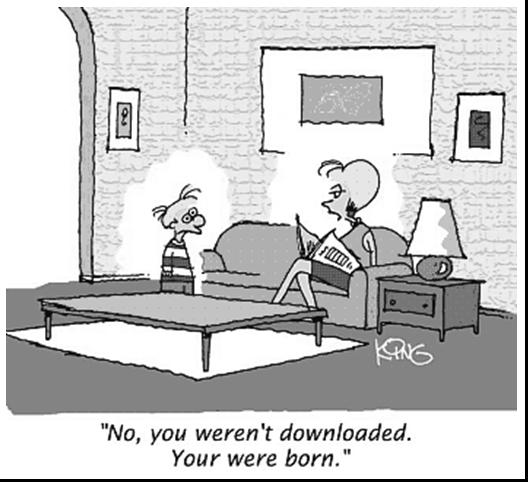
\includegraphics[width=.5\textwidth]{fig1.jpg}
\caption{A typical figure}
\label{fig:exampleFig1}
\end{figure}

\begin{figure}[ht]
\centering
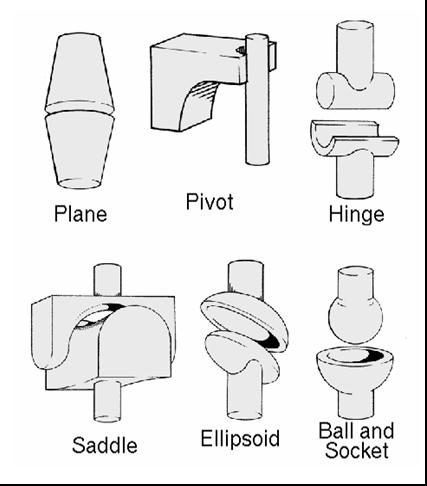
\includegraphics[width=.3\textwidth]{fig2.jpg}
\caption{This figure is an example of a figure caption taking more than one
  line and justified considering margins mentioned in Section~\ref{sec:figs}.}
\label{fig:exampleFig2}
\end{figure}

In tables, try to avoid the use of colored or shaded backgrounds, and avoid
thick, doubled, or unnecessary framing lines. When reporting empirical data,
do not use more decimal digits than warranted by their precision and
reproducibility. Table caption must be placed before the table (see Table 1)
and the font used must also be Helvetica, 10 point, boldface, with 6 points of
space before and after each caption.

\begin{table}[ht]
\centering
\caption{Variables to be considered on the evaluation of interaction
  techniques}
\label{tab:exTable1}
\smallskip
\begin{tabular}{|l|c|c|}
\hline
& Value 1 & Value 2\\[0.5ex]
\hline
&&\\[-2ex]
Case 1 & 1.0 $\pm$ 0.1 & 1.75$\times$10$^{-5}$ $\pm$ 5$\times$10$^{-7}$\\[0.5ex]
\hline
&&\\[-2ex]
Case 2 & 0.003(1) & 100.0\\[0.5ex]
\hline
\end{tabular}
\end{table}

\section{Images}

All images and illustrations should be in black-and-white, or gray tones,
excepting for the papers that will be electronically available (on CD-ROMs,
internet, etc.). The image resolution on paper should be about 600 dpi for
black-and-white images, and 150-300 dpi for grayscale images.  Do not include
images with excessive resolution, as they may take hours to print, without any
visible difference in the result.

\bibliographystyle{sbc}
\bibliography{tumorgrowth}

\end{document}
